\chapter{Electromagnetismo}
\section{Electrostática}
\subsection{Campo eléctrico y ley de Gauss}
\begin{itemize}
\item El campo eléctrico producido por una densidad de carga $\rho(\vb{r})$
es
\begin{align}
\frac{q}{4\pi \epsilon_0}\int \frac{\rho(\vb{r}')}{r^2}\uv{r}dV'.
\end{align}

\item Se define el flujo de campo eléctrico $\vb{E}$ a través de 
una superficie $\mathcal{S}$ como
\begin{align}
\Phi_E\equiv\int _{\mathcal{S}}\vb{E}\vdot d\vb{a}.
\end{align}

\item \textbf{Ley de Gauss:}
\begin{align}
\oint \vb{E}\vdot d\vb{a}=\frac{1}{\ep}q_{\text{enc}},
\end{align}
el flujo de campo eléctrico atravesando una superficie cerrada
es proporcional a la carga que se encuentra encerrada dentro 
de la superficie. La dirección del flujo nos indica si tenemos un 
sumidero o una fuente y, al mismo tiempo, el signo de la carga
encerrada.

\item Es importante aprender a pasar de la forma integral, a la forma
diferencial de la ley de Gauss. Veamos a continuación. 
\begin{align*}
\oint_{\mathcal{S}} \vb{E}\vdot d\vb{a}=\int_{\mathcal{V}}
\qty(\div{\vb{E}})dV
\end{align*}
\textit{\textbf{Paréntesis (teorema de la divergencia)}: la integral 
de superficie cerrada de un campo vectorial es igual a la integral 
de volumen de la divergencia del campo vectorial, integrado sobre
el volumen que encierra la superficie,}

Recordando que 
\begin{align*}
q_{\text{enc}}&=\int_{\mathcal{V}}\rho \ dV,
\end{align*}
por consiguiente, 
\begin{align*}
\int_{\mathcal{V}}\qty(\div{\vb{E}})dV=
\frac{1}{\ep}\int_{\mathcal{V}}\rho \ dV,
\end{align*}
puesto que la integración es sobre el mismo volumen, entonces
los integrandos deben ser iguales,
\begin{align}
\div{\vb{E}}=\frac{\rho}{\ep}.
\end{align}

La ley de Gauss es siempre cierta, \textit{pero no siempre útil}.
Particularmente, las simetrías son cruciales para poder aprovechar 
el resultado establecido en la ley de Gauss:
\begin{enumerate}
\item Simetría esférica: superficie gaussiana una esfera concéntrica.
\item Simetría cilíndrica: superficie gaussiana un cilindro coaxial. 
\item Simetría plana: superficie gaussiana una caja de pastillas.
\end{enumerate}
Aprovecharse de las simetrías $+$ utilizar el principio de superposición
hace que la ley de Gauss se vuelva especialmente útil para su aplicación.

\item $\curl{\vb{E}}=0$. Tomemos el caso de una carga puntual
$q$, cuyo campo eléctrico $E$ es
\begin{align}
\vb{E}=\frac{1}{4\pi\ep}\frac{q}{r^2}\uv{r}.
\end{align}
Ahora calculemos la integral de línea entre dos puntos arbitrarios
$a$ y $b$ del espacio, 
\begin{align*}
\int_a^b \vb{E}\vdot d\vb{l}.
\end{align*}
En coordenadas esféricas, $d\vb{l}=dr\uv{r}
+rd\theta \uv{\boldsymbol{\theta}}+
r\sin\theta d\phi \uv{\boldsymbol{\phi}}$, entonces
\begin{align*}
\int_a^b\vb{E}\vdot d\vb{l}&=\int_a^b\frac{1}{4\pi\ep}\frac{q}{r^2}dr\\
&=\frac{q}{4\pi\ep}\qty(\frac{1}{r_a}-\frac{1}{r_b}),
\end{align*}
por lo tanto, al integrar sobre una trayectoria cerrada la integral 
debe ser igual a cero:
\begin{align}
\oint\vb{E}\vdot d\vb{l}=0.
\end{align}
Por consiguiente, aplicando el teorema de Stokes:
\begin{align}
\oint\vb{E}\vdot d\vb{l}&=\int \qty(\curl{\vb{E}})\vdot d\vb{a}=0\\
\therefore \hspace{5mm} \curl{\vb{E}}&=0.
\end{align}
Este resultado se sigue satisfaciendo para cualquier distribución 
estática de cargas, pues si tenemos $N$ cargas, el campo eléctrico
de la distribución está determinado por 
\begin{align*}
\vb{E}=\vb{E}_1+\vb{E}_2+\ldots+\vb{E}_N\\
\end{align*}
\begin{align}
\therefore \hspace{5mm} 
\curl{\vb{E}}=\curl{\vb{E}_1}+\curl{\vb{E}_2}+\ldots+
\curl{\vb{E}_N}=0,
\end{align}
dado que cada rotor se debe hacer cero.
\end{itemize}
\subsection{Potencial eléctrico}
\begin{itemize}
\item El \textbf{potencial eléctrico} es una función escalar que se define
como
\begin{align}
V(\vb{r})\equiv -\int_{\mathcal{O}}^r\vb{E}\vdot d\vb{l},
\end{align}
con $\mathcal{O}$ un punto de referencia.

\item El teorema fundamental de los gradientes establece que
\begin{align*}
V(\vb{r}_b)-V(\vb{r}_a)=\int_a^b \grad V\vdot d\vb{l},
\end{align*}
por consiguiente, 
\begin{align*}
\int_a^b \grad V\vdot d\vb{l}&=-\int_a^b \vb{E}\vdot d\vb{l}\\
\vb{E}&=-\grad V.
\end{align*}

\item Es una consecuencia de $\curl{\vb{E}}=0$ que las componentes
$E_i$ de $\vb{E}$ no sean completamente independientes entre ellas.
De hecho, la formulación del potencial eléctrico explota al máximo 
esto.

\item \textbf{Ecuación de Poisson:}
\begin{align}
\grad^2V=\frac{\rho}{\ep}.
\end{align}

\item Cálculo del potencial eléctrico $V$ a partir de la distribución de
carga $\rho$:
\begin{align}
\frac{1}{4\pi\ep}\int\frac{\rho(\vb{r}')}{r}\ dV'.
\end{align}

\item \textbf{Discontinuidad al cruzar una superficie de carga $\sigma$}:
supongamos una superficie con densidad superficial de cargar $\sigma$.
Consideremos un área $A$ sobre la superficie, tan pequeña como 
sea necesario para que $\sigma=\text{cte.}$, y apliquemos 
la ley de Gauss con una caja de pastillas gaussiana. Los lados 
de la caja de pastillas (componente paralela a la superficie) no 
contribuyen nada al flujo neto de campo eléctrico, por lo tanto, 
sumando las contribuciones perpendiculares a la superficie se 
tiene $\qty(E_{\text{arriba}}-E_{\text{abajo}})A=\sigma A/\ep$,
entonces $E_{\text{arriba}}-E_{\text{abajo}}=\sigma /\ep$. Por 
lo cual, se concluye que existe una discontinuidad de la componente 
normal de $\vb{E}$ al atravesar una superficie de carga que es igual 
a $\sigma/\ep$. Las componentes paralelas a la superficie son continuas
y es consecuencia directa de 
\begin{align}
\oint \vb{E}\vdot d\vb{l}=0.
\end{align}
No obstante, el potencial eléctrico es continuo a través de cualquier
frontera, ya que 
\begin{align*}
V_{\text{arriba}}-V_{\text{abajo}}=-\int_a^b\vb{E}\vdot d\vb{l};
\end{align*}
conforme la trayectoria entre $a$ y $b$ se hace igual a cero, 
también lo hace el valor de la integral, por consiguiente
\begin{align}
V_{\text{arriba}}=V_{\text{abajo}}.
\end{align}
\end{itemize}

\subsection{Trabajo y energía}
\begin{itemize}
\item De lo que sabemos de mecánica el trabajo sobre un sistema 
para moverlo desde $a$ hasta $b$ es 
\begin{align}
W=\int_a^b\vb{F}\vdot d\vb{l}.
\end{align}
Por consiguiente, el trabajo para mover una carga $q$ es
\begin{align}
W=-q\int_a^b\vb{E}\vdot d\vb{l}=q\qty(V_b-V_a)
\end{align}

\item La energía de una configuración de cargas se define 
como la cantidad de trabajo necesario para armar la configuración:
\begin{align}
W=\frac{1}{2}\sum_i^nq_iV(\vb{r}_i),
\label{eq:ch3-W-point}
\end{align}
donde $V$ es el potencial generado por el resto de las cargas 
en la configuración.

\item Si en vez tenemos una distribución continua de carga $\rho$
entonces podemos reescribir la ecuación \eqref{eq:ch3-W-point}
como
\begin{align}
W=\frac{1}{2} \int \rho Vd\tau.
\end{align}
Si utilizamos la ley de Gauss podemos resscribir esta ecuación como
\begin{align}
W&=\frac{\ep}{2} \int \qty(\div{\vb{E}}) Vd\tau\nonumber\\
&=\frac{\ep}{2}\qty(-\int \vb{E}\vdot \qty(\grad V)d\tau
+\oint V\vb{E}\vdot d\vb{a}),
\end{align}
pero como $\grad V=-\vb{E}$,
\begin{align}
W&=\frac{\ep}{2}\qty(\int E^2d\tau+\oint V\vb{E}\vdot d\vb{a}),
\end{align}
consideramos la integración sobre todo el espacio, y de esa manera,
\begin{align}
W&=\frac{\ep}{2}\int E^2d\tau.
\end{align}
\end{itemize}

\section{Potenciales}
\subsection{El método de imágenes}
\textbf{El problema:} supongamos una carga $q$ que se encuentra a 
una distancia $d$ sobre un plano conductor infinito, ¿cuál es el potencial
en una región por encima del plano?

El punto es establecer cuáles son las condiciones de frontera del problema
y luego encontrar una configuración equivalente que satisfaga dichas 
condiciones de frontera, de esa manera, justificados en el teorema de 
unicidad de las ecuaciones diferenciales, habremos encontrado 
la solución al problema. 

\section{Desplazamiento eléctrico}
\begin{itemize}
\item El efecto de la polarización es producir acumulaciones de carga 
$\rho_b=-\div{\vb{P}}$ dentro del dieléctrico y $\sigma_b=\vb{P}
\vdot \vb{\hat{n}}$ en la superficie. El campo eléctrico debido a la
polarización del medio es justo el campo generado 
por la carga ligada más la carga libre. 
\item Dentro de un dieléctrico, la densidad total de carga 
puede escribirse como 
\begin{align}
\rho=\rho_b+\rho_f,
\end{align}
y, entonces aplicando la ley de Gauss, tenemos 
\begin{align}
\ep \div{\vb{E}}=\rho=\rho_b+\rho_f=-\div{P}+\rho_f,
\end{align}
donde $\vb{E}$ es el campo total.
\begin{align}
\div{\qty(\ep \vb{E}+\vb{P})}=\rho_f.
\end{align}
Así definimos
\begin{align}
\vb{D} \equiv \qty(\ep \vb{E}+\vb{P}),
\end{align}
que se conoce como \textbf{desplazamiento eléctrico}. Por consiguiente, 
en términos de $\vb{D}$ la ley de Gauss se escribe como
\begin{align}
\div{\vb{D}}=\rho_f.
\end{align}
Esta forma de escribir a la ley de Gauss para dieléctricos es particularmente
útil porque solamente considera a la densidad de carga libre.
\item A diferencia del vector de campo eléctrico $\vb{E}$, la componente
paralela a una superficie conductora es discontinua, 
\begin{align}
\vb{D}^{\parallel}_{\text{arriba}}-\vb{D}^{\parallel}_{\text{abajo}}=
\vb{P}^{\parallel}_{\text{arriba}}-\vb{P}^{\parallel}_{\text{abajo}}.
\end{align}
\end{itemize}

\subsection{Dieléctricos lineales}
\begin{itemize}
\item Para muchos sistemas físicos la polarización $\vb{P}$ es directamente 
proporcional al campo eléctrico $\vb{E}$:
\begin{align}
\vb{P}=\ep \chi_e\vb{E},
\end{align}
con $\chi_e$ la susceptibilidad eléctrica del medio, depende 
de la estructura microscópica del medio.

\item En un medio lineal:
\begin{align}
\vb{D}=\ep\vb{E}+\vb{P}=\ep\vb{E}+\ep\chi_e\vb{E}=
\ep\qty(1+\chi_e)\vb{E},
\end{align}
entonces definimos
\begin{align}
\epsilon \equiv  \ep\qty(1+\chi_e).
\end{align}
Por lo tanto,
\begin{align*}
\vb{D}=\epsilon\vb{E}.
\end{align*}
\end{itemize}

\section{Magnetostática}
\subsection{Ley de Biot-Savart}
La electrostática y magnetostática ocurre cuando
\begin{align*}
\pdv{\rho}{t}=0, \hspace{3mm} \pdv{\vb{J}}{t}=0.
\end{align*}
(cargas y corrientes estacionarias.)

\begin{itemize}
\item \textbf{Ley de Biot-Savart} para corrientes estacionarias:
\begin{align}
\vb{B}(\vb{r})=\frac{\mu_0}{4\pi}I\int \frac{d\vb{l}'\cp\vb{\hat{r}}}
{r^2}
\end{align},
donde la integración se realiza a lo largo de trayectoria de la corriente
en la dirección del flujo $d\vb{l}'$.
\begin{align}
\qty[\tx{B}]=\frac{\tx{N}}{\tx{A}\cdot \tx{m}}=\tx{T}.
\end{align}

\item De acuerdo con la ley de Biot-Savart el campo magnético 
alredor de un cable infinito de corriente es 
\begin{align}
\vb{B}=\frac{\mu_0I}{2\pi s} \uv{\phi}.
\end{align}
De primera vista es evidente que $\curl{\vb{B}}\neq 0$,
\begin{align}
\oint \vb{B}\vdot d\vb{l}
= \oint\frac{\mu_0I}{2\pi s}\ dl =\mu_0 I.
\end{align}
Ahora si suponemos que tenemos un manojo de cables de 
corriente, cada uno contribuyendo $\mu_0I$ a la integral de 
$\vb{B}$ alrededor del manojo de cables, entonces la integral 
daría como resultado 
\begin{align*}
\oint \vb{B}\vdot d\vb{l}=\mu_0I_{\tx{enc}},
\label{eq:ampere-inc-law}
\end{align*}
donde $I_\tx{enc}$ es la corriente que encierra una espira 
alrededor de la corriente. También podemos escribir a la corriente
$I$ en términos de la densidad de corriente $\vb{J}$,
\begin{align}
I_{\tx{enc}}=\int \vb{J}\vdot d\vb{a}.
\end{align}
Si aplicamos el teorema de Stokes a la ecuación \eqref{eq:ampere-inc-law}
tenemos
\begin{align}
\int\curl{\vb{B}}\vdot d\vb{a}&=\mu_0\int \vb{J}\vdot d\vb{a}\\
\therefore \hspace{5mm} \curl{\vb{B}}&=\mu_0\vb{J}.
\end{align}
Esta es conocida como la ley de Ampère en forma diferencial.

\item \h{Revisar deducción formal de que la ley de Ampère se cumple 
para cualquier forma de $\vb{J}$,	} \newline
\h{siempre y cuando se cumpla $\div{\vb{J}}=0$.}

\item Similarmente a la ley de Gauss para campos eléctricos, la 
ley de Ampère es útil sólo cuando existen ciertas simetrías:
\begin{enumerate}
\item Líneas infinitas de corriente
\item Planos infinitos
\item Solenoides infinitos
\item Toroides
\end{enumerate}
\end{itemize}

\subsection{Vector potencial magnético}
Que se cumpla que $\div{\vb{B}}$ hace que exista una función 
vectorial de potencial $\vb{A}$ en magnetostática, tal que 
\begin{align}
\vb{B}=\curl{\vb{A}}.
\end{align}
Entonces
\begin{align}
\curl{\vb{B}}=\curl{\curl{\vb{A}}}=\grad{\qty(\div{\vb{A}})}
-\grad^2\vb{A}=\mu_0\vb{J}.
\end{align}
Si imponemos la condición de $\div{\vb{A}}=0$, entonces tenemos 
\begin{align}
\grad^2\vb{A}=-\mu_0\vb{J}.
\label{•}
\end{align}
Esta es simplementa la ecuación de Poisson, cuya solución, 
asumiendo que $\lim_{x\to\infty}\vb{J}=0$,
\begin{align}
\vb{A}(\vb{r})=\frac{\mu_0}{4\pi}\int \frac{\vb{J}(\vb{r}')}{r}\ dV'
\label{}
\end{align}
\subsection{Condiciones de frontera}
\begin{figure}
  \centering
  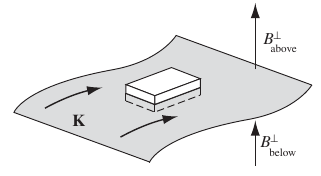
\includegraphics[width=6cm]{images/sup-current.png}
  \caption{Superficie de corriente.}
  \label{fig:sup-current}
\end{figure}
Si consideramos la situación en la \Fref{fig:sup-current} y recordamos que
$\div{\vb{B}}=0$, integramos sobre el volumen de la caja de pastillas,
y aplicamos el teorema de la diverencia 
\begin{align}
\oint \vb{B}\vdot d\vb{a}&=0\\
\qty(B^{\perp}_{\tx{arriba}}-B^{\perp}_{\tx{abajo}})A&=0\\
B^{\perp}_{\tx{arriba}}&=B^{\perp}_{\tx{abajo}}.
\end{align}
Si ahora tomamos una espira, digamos alrededor de una de las caras
de la caja de pastillas y hacemos que la altura de la caja sea 
infinitesimalmente pequeña, tanto como lo necesitemos para 
despreciar la contribución de la componente perpendicular 
del campo magnético, 
\begin{align}
\oint \vb{B}\vdot d\vb{l}&=
\qty(B^{\parallel}_{\tx{arriba}}-B^{\parallel}_{\tx{abajo}})l\\
&=\mu_0I_{\tx{encerrada}}=\mu_0Kl\\
\therefore \hspace{5mm}
B^{\parallel}_{\tx{arriba}}-B^{\parallel}_{\tx{abajo}}&=\mu_0K
\end{align}

\section{El campo auxiliar $\vb{H}$}
Similarmente al efecto de polarización, los campos magnéticos 
en un medio producen el efecto de magnetización, que es 
producir corrientes ligadas $\vb{J}_b=\curl{\vb{M}}$ dentro del 
material y $\vb{K}_b=\vb{M}\cp \uv{n}$ en la superficie. En un 
material magnético, la densidad de corriente total se puede 
escribir como 
\begin{align}
\vb{J}=\vb{J}_b+\vb{J}_f.
\end{align}
Entonces, escribiendo la ley de Ampère
\begin{align}
\frac{1}{\mu_0}\qty(\curl{\vb{B}})&=\vb{J}_b+\vb{J}_f\\
&=\vb{J}_f+\qty(\curl{\vb{M}})\\
\curl{\qty(\frac{1}{\mu_0}\vb{B}-\vb{M})}&=\vb{J}_f,
\end{align}
entonces llamamos $\vb{H}=\frac{1}{\mu_0}\vb{B}-\vb{M}$ y
\begin{align}
\curl{\vb{H}}=\vb{J}_f,
\end{align}
donde $\vb{J}_f$ es la densidad de corriente libre.
\subsection{Condiciones de frontera}
Al atravesar una superficie de corriente en un medio se tiene
\begin{align}
H_{\tx{arriba}}^{\perp}-H_{\tx{abajo}}^{\perp}=
-\qty(M_{\tx{arriba}}^{\perp}-M_{\tx{abajo}}^{\perp})
\end{align}

\section{Medio lineal}
En materiales paramagnéticos y diamagnéticos la magnetización
ocurre sólo mientras existe un campo magnético $\vb{B}$. En muchos 
materiales la magnetización $\vb{M}$ es proporcional a la intensidad 
del campo $\vb{B}$,
\begin{align}
\vb{M}=\chi_m\vb{H},
\end{align}
con $\chi_m$ la susceptibilidad magnética (adimensional).

\begin{align}
\vb{B}&=\mu_0\qty(\vb{H}+\vb{M})\\
\vb{B}&=\mu_0\qty(1+\chi_m)\vb{H}\\
\vb{B}&=\mu\vb{H},
\end{align}
donde $\mu$ se etiqueta como permeabilidad del medio. 
\section{Medios no lineales}
Materiales ferromagnéticos evidencian un comportamiento distinto
al de otro tipo de materiales. Los ferromagnéticos muestran un comportamiento
que se conoce como la curva de histéresis. 


